\documentclass[pl]{minipw} % wszystkie ustawienia szablonu są w minipw.cls; if in English, change [pl] to [en]
\allowdisplaybreaks
\usepackage{indentfirst}
%\usepackage[hidelinks]{hyperref}
\usepackage[all]{nowidow}
\usepackage{caption}
\usepackage{graphicx}
\usepackage{tabularx}
\usepackage{polski}
\usepackage{bm}
\usepackage{amsfonts}
\usepackage{amsmath}
\usepackage[utf8]{inputenc}
\usepackage{indentfirst}
\usepackage{float}
\usepackage{enumitem}
\usepackage{listings}
\setlength{\parindent}{5mm} % wcięcie akapitowe 5mm, zarządzenie Rektora


\begin{document}
\sloppy


% 4. Spis treści
\tableofcontents

% 5. Treść

\cleardoublepage
\pagestyle{fancy}

\chapter*{Wprowadzenie}
%\addcontentsline{toc}{chapter}{Wprowadzenie}
Celem pracy jest przetestowanie ELM na wybranych zestawach danych, przy użyciu służącej do tego, istniejącej już biblioteki do Pythona i~stworzenie własnej implementacji w Matlabie, a następnie przeanalizowanie otrzymanych wyników.

Ahmed Abdelkarim zajmował się porównywaniem wyników dla big data i~small data przy użyciu Pythona.
Aleksandra Hernik sprawdzała dokładność i~wydajność uczenia dla big data za pomocą Matlaba.

\clearpage
\chapter{Opracowanie modelu pracy sieci do ekstremalnego uczenia maszynowego ELM}
\section{Rys historyczny}
Sieci neuronowe znajdują coraz to nowe zastosowania i~stają się jednym z~najważniejszych kierunków rozwoju informatyki. Jednak ograniczeniem tej metody jest długotrwały proces uczenia.

W 2004 roku w~pracy \textit{Extreme Learning Machine: A~New Learning Scheme of Feedforward Neural Networks} \cite{huang-elm-base} Guang-Bin Huang, Qin-Yu Zhu i~Chee-Kheong Siew zaproponowali koncepcję ELM, mającą być rozwiązaniem tego problemu. Publikacja ta dotyczyła zastosowania ELM w~SLFN. Przedstawiała podstawy teoretyczne do zastosowania tej metody, a~także dowodziła zalet tego rozwiązania. Pierwszą z nich jest wspomniana prędkość uczenia. Ponadto w~przeciwieństwie do tradycyjnych opartych na gradientach metod, ELM dąży do minimalizacji norm wag, a~nie tylko błędu, dzięki czemu osiąga lepszą generalizację. Kolejną istotną własnością ELM jest dopuszczanie zastosowania nieróżniczkowalnych funkcji aktywacji (co nie jest możliwe w~tradycyjnych metodach). ELM unika również problemów z~minimami lokalnymi i~przeuczeniem. 

W tym samym roku Guang-Bin Huang i~Chee-Kheong Siew zaproponowali również w~artykule \textit{Extreme Learning Machine: RBF Network Case} \cite{huang-elm-rbf} wariant ELM dla sieci radialnych, których nie dotyczy ta praca. 

Kolejnym istotnym wkładem tych autorów do tematu ELM jest opublikowany w~2005 artykuł \textit{Extreme Learning Machine: Theory and Applications} \cite{huang-elm-tap}. Prezentowane są w~nim wyniki ELM dla testowych danych, które pokazują, że metoda ta pozwala na dobrą klasyfikację, a~może działać nawet kilka tysięcy razy szybciej niż tradycyjne metody.

Z wyżej wymienionymi pracami związane są kontrowersje dotyczące rzeczywistej innowacyjności rozwiązania Huanga i~innych, a~także oskarżenia dotyczące plagiatowania i~nieuwzględniania w~bibliografii rzeczywistych głównych źródeł pracy \cite{originofelm} -- według nich artykuł dotyczący SLFN opiera się głównie na pracy \textit{Feed Forward Neural Networks With Random Weights} Woutera Schmidta, Martina Kraaijvelda i~Roberta Duina z~1992, a~artykuł dotyczący sieci radialnych wzoruje się na \textit{Multivariable Functional Interpolation and Adaptive Networks} Davida Broomheada i~Davida Lowe'a. Huang wskazał pewne różnice między tymi pracami.

W 2015 roku metoda została również ostro skrytykowana przez Yanna LeCuna, jednego z~czołowych specjalistów od sieci neuronowych. Zarzucał on pomysłowi prostotę, wskazywał na jego podobieństwo do wcześniejszych pomysłów i~wątpił w~skuteczność dla większych zestawów danych. Nie odniósł się jednak do wyników zaprezentowanych przez autorów, które pokazują, że rozwiązanie mimo swojej prostoty działa bardzo dobrze.

Teorię o~niedostosowaniu ELM do zastosowań big data podważa wydana kilka miesięcy później praca \textit{High-Performance Extreme Learning Machines: A~Complete Toolbox for Big Data Applications} \cite{akusok-hpelm} autorstwa Antona Akusoka, Kaj-Mikaela Bj\"orka, Yoaba Miche i~Amaury'ego Lendasse. Prezentuje ona obiecujące wyniki zastosowania ELM na big data -- dla testowanych danych błąd jest porównywalny, podczas gdy czas uczenia jest mniejszy (od kilku razy dla niektórych metod, nawet do kilku tysięcy razy dla innych). Praca opisuje również udostępniony przez autorów toolbox, implementujący ELM.

\clearpage
\section{Założenia dla sieci neuronowych klasy ELM}
Rozważane tu ELM zaliczają się do kategorii SLFN -- poza warstwą wejściową i~wyjściową posiadają tylko jedną warstwę ukrytą (patrz rys. \ref{schemat_elm}). Od innych SLFN odróżnia je to, że ELM opierają się na losowym generowaniu neuronów warstwy ukrytej bez późniejszego ich dostosowywania do danych -- dzięki temu, że wszystkie ich parametry, takie jak np. wagi wejściowe, mogą zostać dobrane losowo, są one niezależne od danych trenujących, a~w przeciwieństwie do metody BP, wagi wyjściowe są niezależne od wag wejściowych, co pozwala na nieiteracyjne ich wyznaczenie. Takie rozwiązanie zapewnia o~kilka rzędów wielkości szybszy czas działania od innych metod, takich jak BP, MLP i~SVM \cite{akusok-hpelm}.
\begin{figure}[H]
\centering
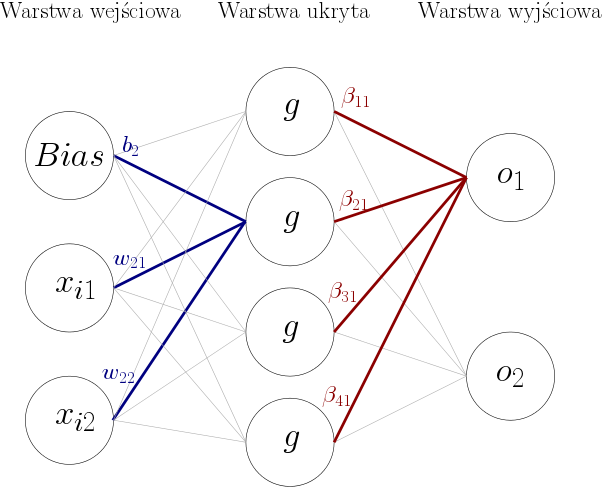
\includegraphics[width=0.9\textwidth]{schemat_sieci.png}
\caption[Schemat SLFN typu ELM]{Schemat SLFN typu ELM (opracowanie własne)}
\label{schemat_elm}
\end{figure}

Niech $N$ to liczba próbek danych trenujących postaci $(\bm{x}_i, \bm{t}_i) \in \mathbb{R}^n \times \mathbb{R}^m$, gdzie $\bm{x}_i = [x_{i1}, x_{i2}, \dots,  x_{in}]^T$ to dane wejściowe, a~$\bm{t}_i = [t_{i1}, t_{i2}, \dots,  t_{im}]^T$ to oczekiwane wyniki. Wtedy dla SLFN z~$\bar{N}$ ukrytymi neuronami wyjście dla i-tej próbki danych $(i=1,\dots,N)$ można zapisać jako:
\begin{equation}
\sum_{j=1}^{\bar{N}} \bm{\beta}_j g (\bm{w}_j \cdot \bm{x}_i + b_j)  = \bm{o}_i,
\end{equation}
gdzie $\bm{w}_j = [w_{j1}, w_{j2},\dots,w_{jn}]^T$ to wektor wag łączących warstwę wejściową z~j-tym neuronem warstwy ukrytej, $\bm{\beta}_j = [\beta_{j1}, \beta_{j2}, \dots, \beta_{jm}]$ to wektor wag łączących j-ty neuron warstwy ukrytej z~warstwą wyjściową, a~$b_j$ to bias. W~przypadku sieci typu ELM, $\bm{w_j}$ i~$\bm{b_j}$ są losowane, tak więc wystarczy wyznaczyć $\bm{\beta_j}$.  W~przypadku przybliżenia z~zerowym błędem otrzymujemy układ $N$ równań $(i=1,\dots,N)$:
\begin{equation}
\sum_{j=1}^{\bar{N}} \bm{\beta}_j g (\bm{w}_j \cdot \bm{x}_i + b_j)  = \bm{t}_i,
\end{equation}
który można zapisać w~postaci macierzowej $\bm{H}\bm{\beta}=\bm{T}$, gdzie: \\
$
H = \begin{bmatrix}
 g(\bm{w}_1 \cdot \bm{x}_1 + b_1) & \cdots & g(\bm{w}_{\bar{N}} \cdot \bm{x}_1 + b_{\bar{N}}) \\
 \vdots & \ddots & \vdots \\
 g(\bm{w}_1 \cdot \bm{x}_N + b_1) & \cdots & g(\bm{w}_{\bar{N}} \cdot \bm{x}_N + b_{\bar{N}})
\end{bmatrix}_{N \times \bar{N}}$, \\
$\bm{\beta} = \begin{bmatrix} \bm{\beta}_1^T \\ \vdots \\ \bm{\beta}_{\bar{N}}^T \end{bmatrix}_{\bar{N} \times m}$ i~
 $ \bm{T} = \begin{bmatrix} \bm{t}_1^T \\ \vdots \\ \bm{t}_N^T \end{bmatrix}_{N \times m}. $\\
W macierzy $\bm{H}$ i-ta kolumna (macierzy wyjścia warstwy ukrytej) to wyjście i-tego neuronu warstwy ukrytej dla $\bm{x}_1, \dots, \bm{x}_N$. Jeśli rozważymy macierz $\bm{W}$ jako macierz odpowiednich wag, $\bm{X}$ jako macierz danych wejściowych i~$\bm{b}$ jako wektor wyrazów wolnych, otrzymujemy $\bm{H} = g(\bm{XW} + \bm{b})$. W~przypadku różnych funkcji aktywacji macierz $\bm{H}$ jest otrzymywana przez konkatenację analogicznie uzyskanych podmacierzy: 
\begin{equation}
\bm{H} = [\bm{H}_1 | \bm{H}_2] = [g_1(\bm{XW}_1 + \bm{b}_1) | g_2(\bm{XW}_2 + \bm{b}_2)]. 
\end{equation}

Sposób rozwiązania równania $\bm{H}\bm{\beta}=\bm{T}$ jest zależny od liczby próbek $N$ i~liczby neuronów warstwy ukrytej $\bar{N}$. W~przypadku, gdy $N \leq \bar{N}$, należy zastosować regularyzację w~celu otrzymania satysfakcjonującej wydajności \cite{akusok-hpelm}. W~najczęstszym przypadku $N \gg \bar{N}$ jednak należy zastosować pseudoinwersję Moore'a-Penrose'a \cite{huang-elm-base}:
\begin{equation}
\bm{H}\bm{\beta}=\bm{T} \implies \bm{\beta}=\bm{H}^{\dagger}\bm{T},
\end{equation}
gdzie 
\begin{equation}
{H}^{\dagger} = (\bm{H}^T \bm{H})^{-1}\bm{H}^T.
\end{equation}
%dodać cytowanie Huanga

Możliwości uczenia się ELM zależą między innymi od doboru funkcji transformacji -- w~szczególności ważne jest, żeby była ona nieliniowa, ponieważ to jedyne miejsce w~całym modelu, w~którym może być wykorzystane jakiekolwiek nieliniowe przekształcenie \cite{akusok-hpelm}. Możliwe jest wykorzystanie różnych funkcji w~różnych neuronach. Dla optymalnej jakości uczenia ważne jest również znormalizowanie danych wejściowych -- jeśli charakterystyki danych wejściowych mają różne rzędy wielkości, relatywnie drobne zmiany większej wartości mogą mieć większe znaczenie niż stosunkowo duże zmiany mniejszych wartości. Normalizacja pozwala na zrównanie wagi zmian wszystkich charakterystyk. \par

W przypadku problemu klasyfikacji, który jest rozważany w~tej pracy, rozwiązaniem jest kategoria, dla której wartość na węźle wyjściowym była największa. 
\section{Wnioski i~uwagi}
Ponieważ ELM jest bardzo szybką metodą, naturalne jest zastosowanie jej do big data -- rozumiejąc big data jako dane takie, że liczba próbek jest wystarczająca, żeby wytrenować sieć bez przeuczania jej, a~ograniczeniem jest tylko czas. W~przypadku small data próbek jest za mało, żeby sieć mogła dokładnie nauczyć się modelu bez przeuczania. Szybkość uczenia w~przypadku big data jest dodatkowo ograniczona sprzętowo -- danych jest zbyt dużo, żeby wszystkie zmieścić do pamięci operacyjnej komputera, co spowalnia dostęp do nich.

\clearpage
\chapter{Wykonanie implementacji ELM w~Pythonie i~Matlabie}
\section{Założenia dotyczące aplikacji}
Projekt polega na przygotowaniu dwóch aplikacji. Pierwsza jest napisana w~języku Python. Druga została stworzona w~środowisku Matlab. Celem obu jest przetestowanie nowego modelu sieci neuronowych -- Extreme Learning Machine. Programy zapewniają możliwość wytrenowania sieci neuronowej przy użyciu różnych danych i~dostarczają informacje, dotyczące czasu trwania i~jakości treningu. Dzięki temu będzie możliwe określenie, czy metoda ELM może być uważana za dobrą alternatywę dla tradycyjnych architektur sieci neuronowych, a~także w~jakich obszarach sprawdzi się najlepiej. Szczególny nacisk został położony na zbadanie działania dla Big Data.

Aplikacje udostępniają następujące funkcjonalności:
\begin{itemize}
\item Przygotowanie danych trenujących i~testowych w~formie plików csv,
\item Trenowanie sieci neuronowej o~architekturze ELM,
\item Klasyfikacja danych testowych przez wytrenowaną sieć,
\item Porównywanie wyników klasyfikacji do spodziewanych rezultatów,
\item Analiza jakości klasyfikacji i~ czasu trwania treningu,
\item Interfejs graficzny.
\end{itemize}
Diagram UML na rysunku \ref{use_case} przedstawia zbiór przypadków użycia aplikacji z~punktu widzenia użytkownika i~systemu, a~w tabeli \ref{use_case_tab} znajduje się ich uszczegółowienie.
\begin{figure}[H]
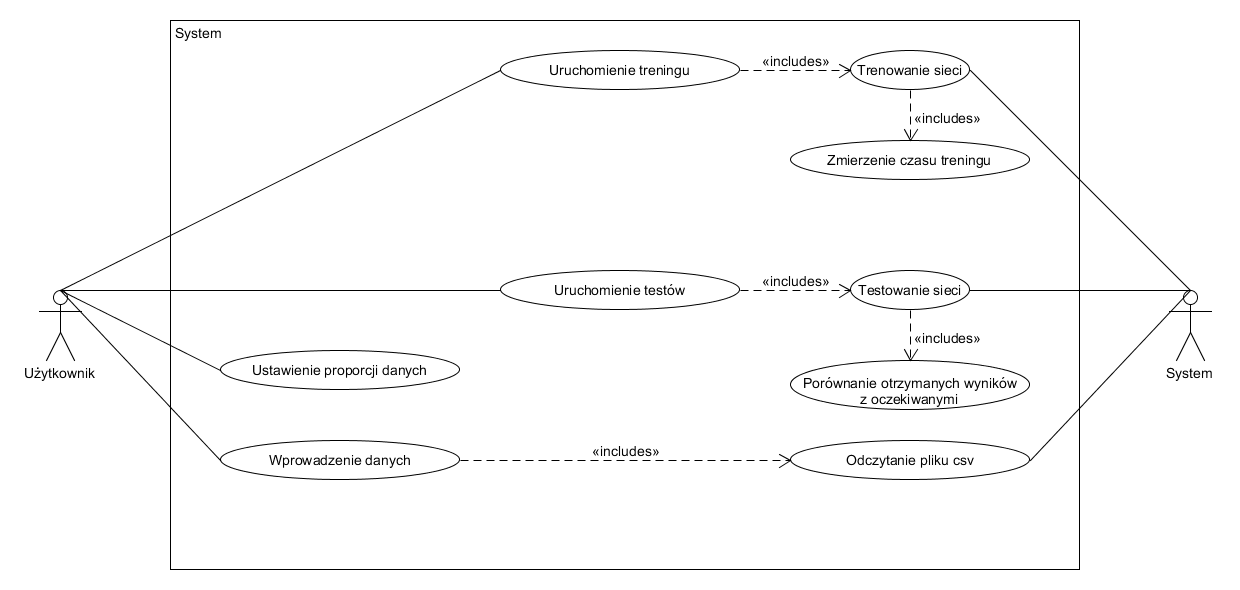
\includegraphics[width=\textwidth]{use_case.png}
\caption[Diagram przypadków użycia]{Diagram przypadków użycia (opracowanie własne)}
\label{use_case}
\end{figure}

\begin{table}[H]
\caption{Opisy przypadków użycia}
\label{use_case_tab}
\centering
\begin{tabular}{|p{3.4cm}|p{5cm}|p{4cm}|}
\hline
\textbf{Nazwa} & \textbf{Opis} & \textbf{Odpowiedź systemu} \\
\hline
Wprowadzenie danych & Wprowadzenie danych używanych do uczenia sieci & Odczytanie pliku csv \\ \hline
Ustawienie proporcji danych & Ustawienie proporcji danych treningowych, testowych i~zatwierdzających & Zapisanie wyboru \\ \hline
Uruchomienie treningu & Uruchomienie treningu sieci schematem ELM & Trenowanie sieci i~zmierzenie czasu treningu \\ \hline
Uruchomienie testów & Uruchomienie testów sieci wytrenowanej wcześniej schematem ELM & Testowanie sieci i~porównanie otrzymanych wyników z~oczekiwanymi \\
\hline
\end{tabular}
\end{table}

Wymagania niefunkcjonalne aplikacji zostały określone w~tabeli \ref{niefunkcjonalne}.
\begin{table}[H]
\caption{Lista wymagań niefunkcjonalnych}
\label{niefunkcjonalne}
\begin{tabular}{|l|l|p{9.4cm}|}
\hline
\textbf{Obszar} & \textbf{Numer} & \textbf{Opis} \\
\hline
Użyteczność & 1 & Aplikacje muszą działać na komputerach wydziałowych \\
 & 2 & Aplikacje powinny mieć przejrzysty interfejs graficzny \\
 & 3 & Wykresy wyświetlane w~aplikacji powinny być czytelne \\
\hline
Wydajność & 4 & Działanie w~oparciu o~ELM powinno dawać o~kilka rzędów wielkości szybszy czas uczenia niż tradycyjne metody \\
\hline 
Inne & 5 & Wykonanie aplikacji w~językach Python i~MATLAB \\
\hline
\end{tabular}
\end{table}
\section{Analiza wykorzystywanych narzędzi}
W związku ze wspomnianą wcześniej pracą \textit{High-Performance Extreme Learning Machines: A~Complete Toolbox for Big Data Applications} Anton Akusok napisał w~Pythonie i~udostępnił dwie biblioteki wykorzystujące ELM, w~tym wykorzystywaną tutaj bibliotekę \textit{HP-ELM} \cite{hpelm}.

Projekt \textit{HP-ELM}, czyli \textit{High Performance toolbox for Extreme Learning Machines} prezentuje kompleksowe podejście do wykorzystania ELM. Zapewnia następujące funkcjonalności:
\begin{itemize}
\item wczytywanie plików z~danymi,
\item tworzenie sieci na podstawie danych,
\item dodawanie neuronów z~wybranymi funkcjami aktywacji (spośród funkcji liniowej, sigmoidalnej, tangensa hiperbolicznego i~funkcji klasy RBF z~różnymi normami),
\item trening sieci,
\item klasyfikacja lub regresja danych przez wytrenowaną sieć,
\item obliczanie błędu średniokwadratowego.
\end{itemize}
Dodatkowo dostępne są liczne udogodnienia:
\begin{itemize}
\item efektywne przechowywanie danych (w~formacie HDF5),
\item możliwość wykorzystywania zbiorów danych niemieszczących się w~pamięci operacyjnej.
\end{itemize}
\section{Projekt aplikacji sieci ELM w~Pythonie}
Aplikacja w~Pythonie wykorzystuje omówioną wcześniej bibliotekę i~dodaje następujące funkcjonalności:
\begin{itemize}
\item normalizację danych,
\item podział danych na treningowe i~testowe,
\item obliczanie procenta poprawnie sklasyfikowanych próbek,
\item pomiar czasu treningu,
\item interfejs graficzny,
\item projektowanie benchmarków i~ich podział na grupy,
\item rysowanie wykresów (zależności błędu średniokwadratowego, procenta sklasyfikowanych próbek i~czasu treningu w~zależności od liczby neuronów) z~podziałem na grupy.
\end{itemize}
Jako dane wejściowe aplikacja przyjmuje dwa pliki -- plik z~danymi wejściowymi oraz plik z~oczekiwanymi wynikami. Oferowane są możliwości przetwarzania dwóch typów plików: \textit{csv} oraz \textit{hdf5}. 

\textit{Csv} to najczęstszy format stosowany do danych tego typu -- informacje są wczytywane za pomocą biblioteki \textit{numpy} \cite{numpy} (która jest również wykorzystywana do ogólnego przetwarzania macierzy, na przykład przy wyznaczaniu błędu) do pamięci jako macierz, którą dalej biblioteka \textit{HP-ELM} jest już w~stanie bezpośrednio przetwarzać. Ograniczeniem (w~celu utrzymania prostoty interfejsu) jest wymóg, aby dane były oddzielone przecinkami -- jednak nie powinno być to problemem ze względu na liczbę powszechnie stosowanych aplikacji pozwalających dostosować te pliki (np. pakiet \textit{Office}). Dane wczytane z~plików \textit{csv} są traktowane jako \textit{small data} i~wykorzystują implementację wczytującą dane do pamięci w~całości. 

\textit{Hdf5} (rozszerzenie \textit{h5}) to format zaprojektowany w~celu przechowywania i~organizowania dużych ilości danych \cite{hdf5}. Biblioteka \textit{HP-ELM} przyjmuje tylko specyficzne pliki \textit{hdf5} i~nie wykorzystuje wszystkich możliwości tego formatu (dotyczących organizacji). Narzucona jest prosta struktura, w~której dane znajdują się w~zbiorze o~nazwie \textit{data} -- jednak nic więcej nie jest potrzebne do wykorzystania ELM. W~celu odczytywania i~przetwarzania plików \textit{hdf5} wykorzystywana jest biblioteka \textit{h5py} \cite{h5py}. Dane wczytane jako \textit{hdf5} traktowane są jako \textit{big data} i~przetwarzane są bez wczytywania całości danych do pamięci, co umożliwia przetwarzanie zbiorów danych, które przekraczają rozmiarem ilość dostępnej pamięci RAM. Udostępniona została możliwość konwersji plików \textit{csv} na pliki \textit{hdf5} zgodne z~aplikacją, co pozwala zasymulować działanie \textit{big data} nawet dla niewielkich zbiorów danych.  

Do normalizacji została użyta biblioteka \textit{sklearn} \cite{sklearn} -- o~ile implementacja własnej normalizacji jest prosta, lepszym pomysłem jest wykorzystanie sprawdzonego rozwiązania.

Interfejs graficzny został stworzony z~wykorzystaniem biblioteki \textit{Tkinter}. Oprócz wczytania danych i~uruchomienia umożliwia on projektowanie benchmarków i~łączenie ich w~grupy. Możliwe jest dodawanie neuronów, których funkcja aktywacji jest jedną z~predefiniowanych funkcji udostępnionych w~bibliotece \textit{HP-ELM}. W~jednym benchmarku mogą zostać wykorzystane neurony z~różnymi funkcjami aktywacji. 

Funkcjonalność łączenia benchmarków w~grupy została wprowadzona w~celu umożliwienia tworzenia wykresów porównujących na przykład różne funkcje aktywacji. Dane wyjściowe benchmarków znajdujących się w~tej samej grupie zostaną potraktowane jako pojedyncza seria danych przy rysowaniu wykresu -- tak więc stworzenie kilku grup pozwala na otrzymanie kilku serii danych na jednym wykresie, co jest przydatne szczególnie w~celu porównywania wyników. 

Na rysunku \ref{przykladowy} jest przedstawiony przykładowy wykres zależności procenta poprawnie przewidzianych klas w~zależności od liczby neuronów dla dwóch grup -- grupa 1 składa się z~czterech benchmarków zawierających jedynie neurony z~sigmoidalną funkcją aktywacji, a~w skład grupy 2 wchodzą cztery benchmarki, w~których neurony oparte są o~tangens hiperboliczny. 
 
\begin{figure}[H]
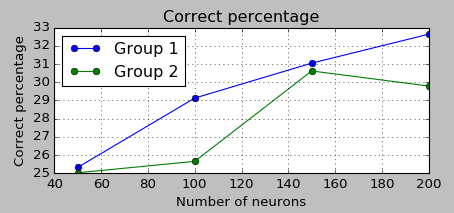
\includegraphics[width=\textwidth]{przykladowy_wykres.png}
\caption[Przykładowy wykres z~dwiema grupami danych]{Przykładowy wykres z~dwiema grupami danych (opracowanie własne)}
\label{przykladowy}
\end{figure}


Wykresy są rysowane przy użyciu biblioteki \textit{matplotlib} i~są ostatecznym rezultatem działania programu.

\section{Dokumentacja kodu w~Pythonie}
Aplikacja sieci ELM w~Pythonie składa się z~plików:
\begin{itemize}
\item \textit{benchmark.py},
\item \textit{error.py}, 
\item \textit{preprocessor.py},
\item \textit{test.py}.
\end{itemize}
Ponadto wykorzystywane są biblioteki:
\begin{itemize}
\item \textit{HP-ELM}
\item \textit{numpy}
\item \textit{sklearn}
\item \textit{h5py}
\item \textit{matplotlib}
\end{itemize}
Plik \textit{test.py} to główny plik aplikacji, w~którym zdefiniowane jest rozmieszczenie interfejsu użytkownika oraz funkcje wywoływane przy naciśnięciu odpowiednich jego elementów, takie jak zapamiętywanie dodanych neuronów, uruchomienie testu i~rysowanie wykresów.

W pliku \textit{preprocessor.py} znajduje się zestaw funkcji odpowiedzialnych za wstępne przetwarzanie danych:
\begin{itemize}
\item \textbf{open\textunderscore csv}(\textit{path}) -- otwiera plik \textit{csv} (rozdzielony przecinkami) ze ścieżki \textit{path} i~zwraca utworzoną na jego podstawie macierz
\item \textbf{normalize}(\textit{data}) -- zwraca znormalizowane dane z~macierzy \textit{data}
\item \textbf{normalize\textunderscore hdf5}(\textit{data\textunderscore path}, \textit{output\textunderscore path}) -- normalizuje dane z~pliku \textit{data\textunderscore path} w~formacie \textit{hdf5} do pliku \textit{output\textunderscore path}.
\item \textbf{split}(\textit{data}, \textit{results}, \textit{training\textunderscore percentage}) -- dzieli dane wskazane w~macierzy \textit{data} i~\textit{results} na dane i~rezultaty treningowe oraz testowe w~zależności od \textit{training\textunderscore percentage}, zwraca dane treningowe, dane testowe, rezultaty treningowe i~rezultaty testowe.
\item \textbf{split\textunderscore hdf5}(\textit{data\textunderscore path}, \textit{results\textunderscore path}, \textit{training\textunderscore percentage}, \textit{training\textunderscore data\textunderscore path}, \textit{test\textunderscore data\textunderscore path}, \textit{training\textunderscore results\textunderscore path}, \textit{test\textunderscore results\textunderscore path}) -- analogicznie do funkcji \textbf{split} dzieli dane znajdujące się w~plikach \textit{hdf5} do odpowiednich plików wynikowych.
\end{itemize}
Plik \textit{error.py} rozszerza funkcjonalność biblioteki \textit{HP-ELM} o~dodatkowy sposób liczenia błędu klasyfikacji za pomocą funkcji:
\begin{itemize}
\item \textbf{percentage}(\textit{expected}, \textit{actual}) -- zwraca procent poprawnie sklasyfikowanych próbek na podstawie macierzy \textit{expected} (oczekiwane wyniki) i~\textit{actual} (rzeczywiste wyniki).
\item \textbf{hdf5\textunderscore percentage}(\textit{expected\textunderscore path}, \textit{actual\textunderscore path} -- analogicznie do funkcji \textbf{percentage}, dla wskazanych plików \textit{hdf5}.
\end{itemize}

W pliku \textit{benchmark.py} zdefiniowana została klasa \textbf{Benchmark}, która automatyzuje uruchamianie testów i~ma następujące metody:
\begin{itemize}
\item \textbf{\textunderscore \textunderscore init\textunderscore \textunderscore}(\textit{self}, \textit{name}, \textit{training\textunderscore percentage}, \textit{neurons}) -- konstruktor, tworzący instancję klasy \textbf{Benchmark} z~uzupełnionymi odpowiednimi polami. Nie powinien być wywoływany bezpośrednio.
\item \textbf{small\textunderscore benchmark}(\textit{name}, \textit{training\textunderscore percentage}, \textit{neurons}, \textit{data}, \textit{results}) -- statyczna metoda tworząca obiekt klasy \textbf{Benchmark} przystosowany do obliczeń small data (na macierzach w~pamięci, wczytanych z~plików \textit{csv}). Ustawia nazwę, procent danych treningowych, zestaw benchmarków (listę zawierająca zestawy neuronów dla każdego z~nich), dane i~oczekiwane wyniki.
\item \textbf{big\textunderscore benchmark}(\textit{name}, \textit{training\textunderscore percentage}, \textit{neurons}, \textit{data\textunderscore path}, \textit{results\textunderscore path}, \textit{output\textunderscore path}) -- statyczna metoda działająca analogicznie do \textbf{small\textunderscore benchmark}, ale dla obliczeń big data (na plikach \textit{hdf5}). 
\item \textbf{run}(\textit{self}) -- uruchamia benchmark i~zwraca błędy średniokwadratowe, procent poprawnie sklasyfikowanych danych i~czas trwania treningu.
\end{itemize}
\clearpage
\section{Projekt aplikacji sieci ELM w~Matlabie}
W Matlabie powstała pełna implementacja algorytmów ELM w~formie klasy, zawierającej wszystkie niezbędne funkcje.
Pozwala na trenowanie i~testowanie sieci dla wybranej liczby neuronów z~dowolnymi funkcjami aktywacji. 
W celu umożliwienia maksymalnej elastyczności korzystanie z~aplikacji polega na wywoływaniu kolejnych funkcji klasy.
Został przygotowany skrypt, zawierający przykładowe wykonanie algorytmu.
Możliwa jest jego modyfikacja zgodnie z~własnymi potrzebami i~pomysłami.

Algorytm można podzielić na kilka etapów.
Najpierw konieczne jest utworzenie obiektu sieci, który jest inicjalizowany zbiorem danych, takich, że $n-1$ kolumn to kolejne cechy, a~ostatnia kolumna oznacza klasy.
Na przykład w~macierzy:
\[D= \begin{bmatrix} 3&5&0&1 \\ 1&8&1&4 \\ 1&3&0&1 \\ 0&1&0&2 \end{bmatrix}\]
pierwsza obserwacja składa się z~cech o~wartościach 3, 5 i~0 i~należy do klasy 1.

Tak może wyglądać wywołanie funkcji inicjalizującej sieć:
\begin{lstlisting}
	>> network = ELM(D, 90);
\end{lstlisting}
Pierwszy argument to macierz danych, a~drugi -- procent danych trenujących.

Zbiór danych jest dzielony na część treningową i~testową, zgodnie z~wartością podaną przy tworzeniu sieci. 
Ponadto dane są dzielone na dwie części -- macierz cech i~wektor klas.
Wektor klas jest przekształcany w~macierz o~wysokości równej liczbie obserwacji i~szerokości równej liczbie klas.
Macierz ta jest wypełniona zerami z~wyjątkiem jednego miejsca w~każdym wierszu -- w~kolumnie o~numerze równym numerowi klasy, do której należy dana obserwacja, wpisane jest 1.
Na przykład dla wektora:
\[ \begin{bmatrix} 1 \\ 4 \\ 1 \\ 2 \end{bmatrix}\]
powstanie macierz:
\[ \begin{bmatrix} 1&0&0&0 \\ 0&0&0&1 \\ 1&0&0&0 \\ 0&1&0&0 \end{bmatrix}.\]
Można zauważyć, że prosta modyfikacja pozwoliłaby na przyjmowanie zbiorów danych, w~których jedna obserwacja należy w~różnym stopniu do kilku klas.

Ukrytym (odbywającym się podczas inicjalizacji obiektu klasy) etapem przygotowywania danych jest ich normalizacja. 
Polega ona na sprowadzeniu wartości wszystkich cech do przedziału $[0, 1]$, korzystając z~wzoru:
\[(element - min(kolumna))/(max(kolumna) - min(kolumna)).\]

Następnie muszą zostać dodane neurony.
Dodanie neuronów polega na wywołaniu funkcji, przyjmującej dwa argumenty -- liczbę neuronów i~funkcję aktywacji.
W przeciwieństwie do aplikacji w~Pythonie, opisywana implementacja pozwala na wykorzystanie dowolnej funkcji.
Na przykład wywołanie funkcji:
\begin{lstlisting}
	>> network.addNeurons('sin(x)', 50);
\end{lstlisting}
spowoduje dodanie 50 neuronów z~funkcją aktywacji sinus.

Gdy zostaną dodane neurony można rozpocząć uczenie sieci. 
Składają się na nie przygotowanie macierzy na podstawie danych i~neuronów i~pseudoinwersja tej macierzy. 
Gdy sieć jest nauczona, można rozpocząć klasyfikację danych testowych.
Algorytmy treningu i~klasyfikacji zostały dokładniej opisane w~rozdziale 1.2.
Pośrednim wynikiem klasyfikacji jest macierz o~wymiarach: liczba klas na liczbę obserwacji.
Dla każdej obserwacji zawiera ona wartości informujące o~tym, w~jakim stopniu należy ona do każdej z~klas.
Aby wynikiem dla każdej obserwacji była jedna klasa, wybierana jest klasa, dla której ta wartość jest największa.
Na przykład jeśli pośrednim wynikiem była macierz:
\[ \begin{bmatrix} 1&4&2&6 \\ 3&1&0&1 \\ 2&8&4&3 \\ 3&1&1&1 \end{bmatrix},\]
to ostatecznym wynikiem będzie wektor:
\[ \begin{bmatrix} 4 \\ 1 \\ 2 \\ 1 \end{bmatrix}.\]

Następnie wyniki otrzymane można porównać z~oczekiwanymi za pomocą dwóch funkcji: średnia odległość od poprawnego wyniku i~procent trafień.

\section{Dokumentacja kodu w~Matlabie}
Aplikacja sieci ELM w~Matlabie składa się z~dwóch plików: \textit{ELM.m}, zawierającego implementację sieci neuronowej, oraz skryptu \textit{ELM\textunderscore run.m}, służącego jako przykładowe wywołanie -- opisany dokładnie został w~instrukcji użytkownika.

W pliku \textit{ELM.m} zaimplementowana została klasa \textbf{ELM}, która zapewnia wszystkie funkcjonalności biblioteki. Zawiera metody:
\begin{itemize}
\item \textbf{ELM}(\textit{data}, \textit{trainingPercentage}) -- tworzy obiekt klasy ELM z~danymi \textit{data} -- macierzą, która w~ostatniej kolumnie zawiera oczekiwane wyniki, dzieląc je na dane treningowe i~testowe według \textit{trainingPercentage}.
\item \textbf{addNeurons}(\textit{obj}, \textit{funcStr}, \textit{num}) -- dodaje do sieci \textit{num} neuronów z~funkcją aktywacji opisaną w~\textit{funcStr} (napis opisujący dowolną funkcję od zmiennej x, na przykład 'x * x').  
\item \textbf{normalize}(\textit{\~}, \textit{data}) -- zwraca znormalizowane dane z~macierzy \textit{data}.
\item \textbf{train}(\textit{obj}) -- trenuje sieć.
\item \textbf{predict}(\textit{obj}) -- uruchamia test (wymaga uprzedniego wytrenowania sieci).
\item \textbf{exactCompare}(\textit{\~}, \textit{actualT}, \textit{predictedT}) -- zwraca część (liczbę od 0 do 1) poprawnie sklasyfikowanych próbek, gdzie \textit{actualT} i~\textit{predictedT} to odpowiednio rzeczywiste i~otrzymane wyniki.
\item \textbf{meanDistanceCompare}(\textit{\~}, \textit{actualT}, \textit{predictedT}) -- zwraca średni moduł z~różnicy między rzeczywistymi i~otrzymanymi wynikami.
\item \textbf{parseData}(\textit{\~}, \textit{d}) -- przetwarza macierz \textit{d}, zwracając \textit{X} -- dane wejściowe i~\textit{T} -- oczekiwane wyniki, znajdujące się w~ostatniej kolumnie \textit{d}.
\item \textbf{createH}(\textit{obj}, \textit{X}) -- wyznacza macierz \textit{H}, używaną w~wewnętrznych obliczeniach ELM.
\end{itemize}
\clearpage
\section{Aplikacje w~Matlabie i~Pythonie -- różnice}
\label{porownanie_aplikacji}
Implementacje algorytmu w~obu aplikacjach różnią się. 
Niektóre z tych różnic mogą być przyczyną rozbieżności w~wynikach aplikacji.
Główne różnice są następujące:
\begin{enumerate}
\item W~dokumentacji biblioteki w~Pythonie nie zostało wspomniane wykorzystywanie wyrazów wolnych w~sieci.
W Matlabie są one losowane i~wykorzystywane podczas uczenia.
\item Zastosowano różne algorytmy normalizacji danych.
\item W~Matlabie nie występuje ograniczenie na liczbę neuronów liniowych.
\item W~obu implementacjach została stworzona funkcja wyliczająca procent trafionych danych, ale każda aplikacja ma również po jednej dodatkowej funkcji -- w~Pythonie błąd średniokwadratowy, w~Matlabie suma modułów różnicy prawidłowej i~otrzymanej odpowiedzi.
\item W~Pythonie możliwy jest wybór wyłącznie z~predefiniowanych funkcji aktywacji. 
W Matlabie można wprowadzić dowolną funkcję, co daje większe możliwości, ale nakłada na użytkownika obowiązek zadbania o~to, żeby podana funkcja spełniała założenia ELM.
\end{enumerate}

\section{Wnioski i~uwagi}
\begin{itemize}
\item Automatyczne testy, sprawdzające główną funkcjonalność programu -- trening sieci -- nie zostaną utworzone. Istotą projektu jest przeanalizowanie otrzymywanych, a~nie otrzymanie z~góry zaplanowanych wyników.
\item Nie zostały postawione wymagania związane z~niezawodnością i~utrzymaniem. Aplikacje służą wyłącznie jako narzędzia do przetestowania nowej technologii, więc jedynym wymaganiem jest działanie w~momencie przeprowadzania testów. Ta kwestia może ulec zmianie, jeśli testy wypadną korzystnie dla ELM.
\item Wydajność jest raczej oczekiwaniem, nie wymaganiem. Z~prac, na których bazuje projekt wynika, że metoda powinna być szybka, jednak założenia projektu polegają na sprawdzeniu, a~nie przyjęciu tej tezy. Ponadto nie zostały zaimplementowane inne metody uczenia sieci neuronowych, więc precyzyjna ocena wydajności byłaby trudna.
\item Funkcjonalność normalizacji danych oferowana przez wykorzystywaną bibliotekę \textit{HP-ELM} nie działa (po jej zastosowaniu dane nie zmieniają się) i~została zastąpiona inną implementacją, która nieznacznie poprawia wyniki.
\item Biblioteka \textit{HP-ELM} nie pozwala na dodanie liczby neuronów liniowych większej od liczby cech próbek -- na przykład w~przypadku próbki z~50 cechami próba dodania 2000 neuronów liniowych skończy się faktycznym dodaniem jedynie 50, o~czym dokumentacja biblioteki nie wspomina.
\item W~aplikacji sieci ELM w~Pythonie, w~przypadku danych typu \textit{hdf5}, ze względu na konieczność przetwarzania danych na dysku, tworzone są pliki pośrednie -- dla pliku o~nazwie \textit{plik.h5}, w~katalogu \textit{plik\textunderscore test\textunderscore results/plik/} powstaną pliki:
\begin{itemize}
\item \textit{plik\textunderscore normalized.h5}, zawierający pełne dane po normalizacji, 
\item \textit{plik\textunderscore training\textunderscore data.h5}, zawierający wydzielone dane trenujące, 
\item \textit{plik\textunderscore test\textunderscore data.h5}, zawierający wydzielone dane testowe,
\item \textit{plik\textunderscore training\textunderscore results.h5}, zawierający wyniki dla danych trenujących,
\item \textit{plik\textunderscore test\textunderscore expected.h5}, zawierający oczekiwane wyniki dla danych testowych,
\item \textit{plik\textunderscore test\textunderscore output.h5}, zawierający otrzymane wyniki dla danych testowych.
\end{itemize} 
Nie są one usuwane automatycznie, gdyż umożliwiają dokładniejszy wgląd w~działanie aplikacji. Są jednak nadpisywane bez ostrzeżenia przy ponownym uruchomieniu programu.
\end{itemize}
\clearpage
\chapter{Trening ELM dla wybranych benchmarków big data i~small data}
\section{Założenia}
We wszystkich dalszych testach przyjęte zostało 80\% danych treningowych. Do testów wydajności dostępne były dwa zestawy:
\begin{enumerate}
\item AMD Phenom II X4 965 @ 3.4 GHz, 16 GB RAM,
\item Intel Core i5 4200M @ 2.5 GHz, 8 GB RAM.
\end{enumerate}
Zestaw 1 był używany przy testach aplikacji w~Pythonie, a~zestaw 2 przy testach aplikacji w~Matlabie.
\section{Przewidywanie wyniku meczu w~grze \textit{Dota 2}}
\subsection{Opis}
\textit{Dota 2} to internetowa, drużynowa gra komputerowa, w~której dwa pięcioosobowe zespoły, nazwane \textit{Radiant} i~\textit{Dire}, starają się zniszczyć bazę przeciwnika. Każda rozgrywka kończy się zwycięstwem dokładnie jednej z~dwóch drużyn -- remisy nie są możliwe. W~celu zniszczenia głównej bazy przeciwnika, oznaczonej na mapie (rysunek \ref{dota2_map}) gwiazdką, trzeba zniszczyć dwie wieże (oznaczone kółkiem) znajdujące się bezpośrednio przy niej, a~także wszystkie przeciwne wieże i~koszary (oznaczone trójkątem) na przynajmniej jednej z~trzech widocznych ścieżek.

\begin{figure}[H]
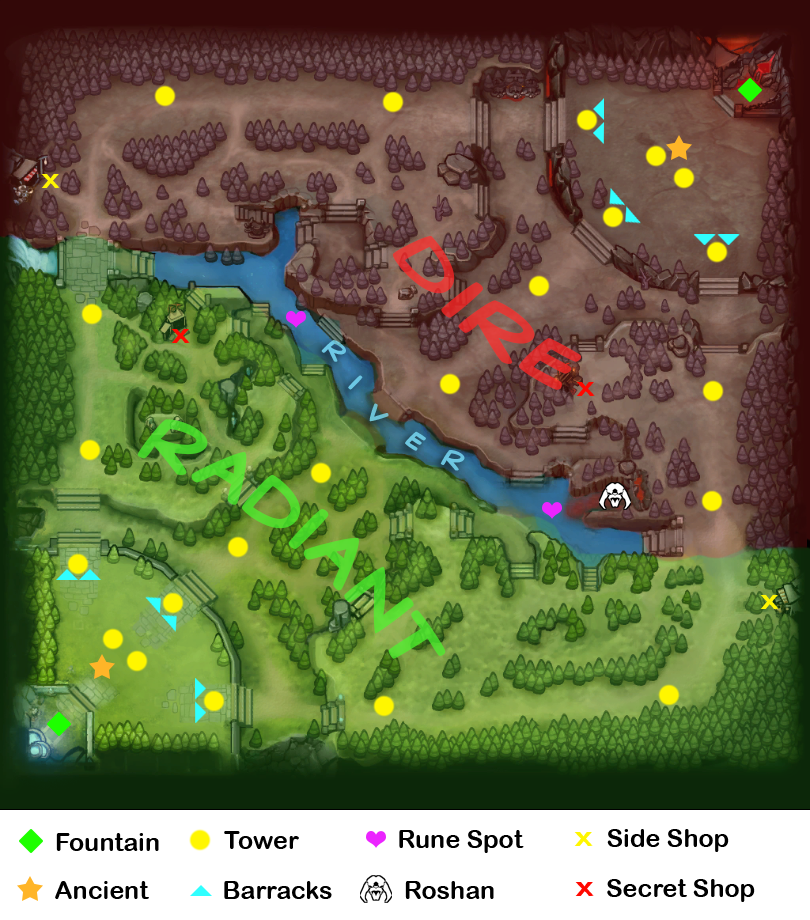
\includegraphics[width=\textwidth]{dota2_map.png}
\caption[Opisana mapa w~grze \textit{Dota 2}]{Opisana mapa w~grze \textit{Dota 2} \cite{dota2_map_src}} 
\label{dota2_map}
\end{figure}

Dane dotyczące meczów w~grze \textit{Dota 2} zostały udostępnione przez Devina Anzelmo na stronie Kaggle \cite{dota2}. Struktura danych jest relacyjna -- czyli bez wstępnego przetworzenia zbyt złożona dla ELM -- więc w~eksperymentach została wykorzystana tylko część danych. Zbiór danych obejmuje 50000 próbek, gdzie każda próbka charakteryzuje jeden mecz.  Wynikiem dla każdej próbki jest jedna z~dwóch klas -- 0, gdy wygrała drużyna \textit{Dire} i~1, gdy wygrała drużyna \textit{Radiant}. Próbki zawierają następujące cechy każdego meczu:
\begin{enumerate}
\item czas trwania meczu,
\item status wież należących do drużyny \textit{Radiant}, zakodowany w~16-bitowej liczbie całkowitej,
\item status wież należących do drużyny \textit{Dire},
\item status koszarów należących do drużyny \textit{Dire}, zakodowany w~8-bitowej liczbie całkowitej,
\item status koszarów należących do drużyny \textit{Radiant},
\item czas pierwszego zabójstwa,
\item tryb gry, zapisany jako wartości od 1 do 22,
\item liczba negatywnych głosów oddanych przez graczy na dany mecz,
\item liczba pozytywnych głosów oddanych przez graczy na dany mecz,
\item grupa serwerów, na których rozgrywany był mecz.
\end{enumerate}
Więcej informacji dotyczących danych jest dostępna na stronie będącej źródłem danych \cite{dota2}, a~wyjaśnienia dotyczące struktury danych (na przykład kodowanie statusu wież) są dostępne w~dokumentacji WebAPI gry \textit{Dota 2} \cite{dota2_webapi}. W~tabeli \ref{dota2_first_5} przedstawione jest 5 przykładowych nieznormalizowanych próbek, zgodnych z~powyższym opisem.
\begin{table}[H]
\caption{Przykładowe dane do przewidywania zwycięzcy}
\label{dota2_first_5}
\centering
\begin{tabular}{|c|c|c|c|c|c|c|c|c|c|}
\hline
\textbf{1} & \textbf{2} & \textbf{3} & \textbf{4} & \textbf{5} & \textbf{6} & \textbf{7} & \textbf{8} & \textbf{9} & \textbf{10} \\
\hline
2375 & 1982 & 4 & 3 & 63 & 1 & 22 & 0 & 1 & 155 \\
2582 & 0 & 1846 & 63 & 0 & 221 & 22 & 0 & 2 & 154 \\
2716 & 256 & 1972 & 63 & 48 & 190 & 22 & 0 & 0 & 132 \\
3085 & 4 & 1924 & 51 & 3 & 40 & 22 & 0 & 0 & 191 \\
1887 & 2047 & 0 & 0 & 63 & 58 & 22 & 0 & 0 & 156 \\
\hline
\end{tabular}
\end{table}

Ten zestaw danych można uznać za łatwy, ponieważ ze względu na opisany wcześniej charakter rozgrywki, w~większości przypadków sam status wież należących do danej drużyny jest wystarczającym wskaźnikiem zwycięstwa -- drużyna, która straciła wszystkie swoje wieże, wygrywa bardzo rzadko.
\subsection{Trening sieci ELM w~Pythonie}
Niezależnie od wyboru funkcji aktywacji, nawet przy liczbach neuronów tak niskich jak 10, po wytrenowaniu poprawnie sklasyfikowanych zostało około 99\% meczów, a~dodawanie większej ich liczby jedynie wydłuża czas treningu. 

Na rysunku \ref{wyniki_dota2_python} grupa 1 to benchmarki wykorzystujące sigmoidalną funkcję aktywacji, a~benchmarki z~grupy 2 używały tangensa hiperbolicznego.

\begin{figure}[H]
\centering
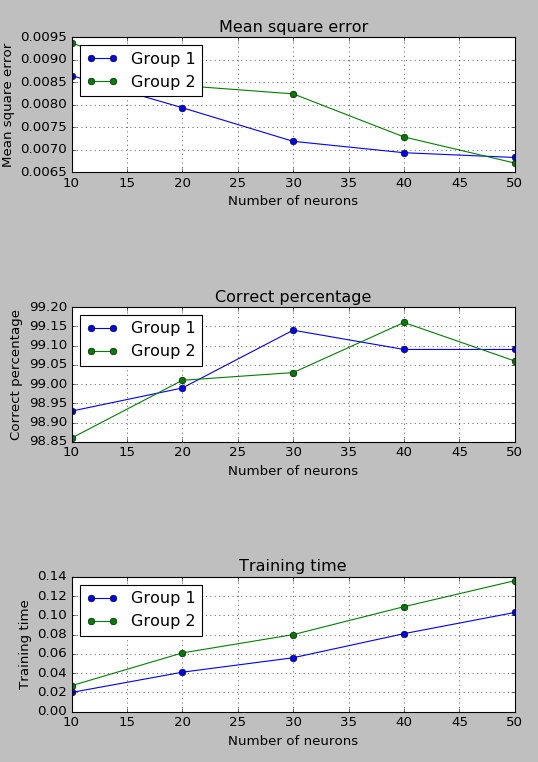
\includegraphics[width=0.8\textwidth]{wyniki_dota2_python.png}
\caption[Wyniki dla niewielkiej liczby neuronów]{Wyniki dla niewielkiej liczby neuronów (opracowanie własne)}
\label{wyniki_dota2_python}
\end{figure}
Jak widać, różnica między funkcjami jest bardzo niewielka. Zwiększanie liczby neuronów również nie wpływa zauważalnie na rozwiązanie. Czas treningu, zgodnie z~zapewnieniami twórców ELM, jest bardzo niewielki -- wszystkie pokazane tu benchmarki zajęły łącznie mniej niż sekundę, mimo dużej liczby danych trenujących. 


Na rysunku \ref{wyniki_dota2_python_performance} uwzględniona została tylko funkcja sigmoidalna, na większej liczbie neuronów.
\begin{figure}[H]
\centering
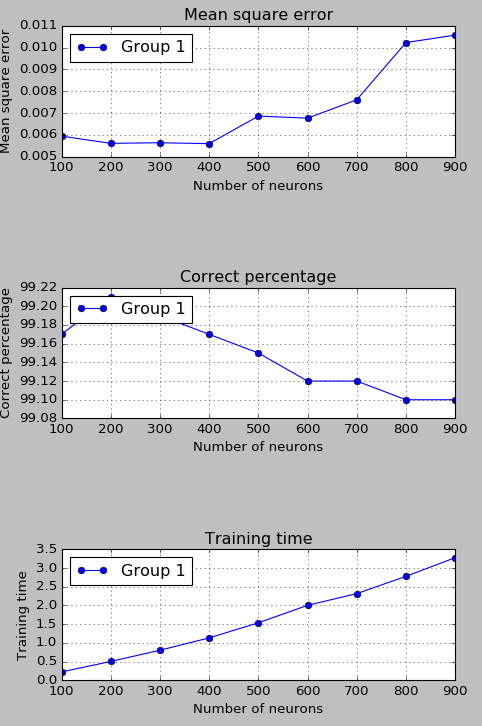
\includegraphics[width=0.8\textwidth]{wyniki_dota2_python_performance.png}
\caption[Wyniki dla dużej liczby neuronów liczby neuronów]{Wyniki dla dużej liczby neuronów liczby neuronów (opracowanie własne)}
\label{wyniki_dota2_python_performance}
\end{figure}
Jak widać, dodawanie neuronów przy większych wartościach wciąż nie zwiększyło jakości treningu, a~wręcz przeciwnie -- neurony dodane powyżej 200 zaczęły już tylko pogarszać wyniki. Zależność czasu trwania treningu od liczby neuronów jest liniowa przy takich rzędach wielkości neuronów. Dla 900 neuronów (i~40000 próbek danych treningowych) czas treningu to niewiele ponad 3 sekundy -- tak więc główna cecha wyróżniająca ELM, czyli wydajność, jest widoczna również dla większych problemów. Przy znaczącym zwiększeniu liczby neuronów -- z~900 do 10000 -- okazało się, że liniowa zależność jest jedynie pozorna, gdyż obliczenia nie skończyły się po 10 minutach, a~w przypadku liniowej relacji trening nie powinien trwać dłużej niż minutę.
\label{10000_dota2}

\subsection{Trening sieci ELM w~Matlabie}
Na rysunku \ref{dota_liczba_neuronow} została przedstawiona skuteczność uczenia dla funkcji aktywacji sigmoidalnej i~tangensa hiperbolicznego.
Można zauważyć, że najlepsze wyniki są otrzymywane dla liczby neuronów od 50 do 300.
Powyżej 300 rezultaty są gorsze, niektóre znacząco.
Jednak najlepsze wyniki są zadowalające -- niektóre ponad 99\%.
\begin{figure}[H]
\centering
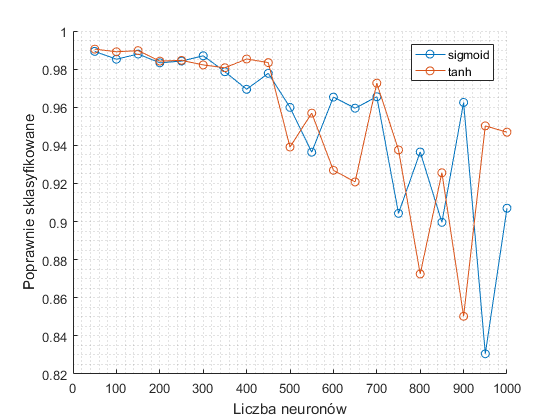
\includegraphics[width=\textwidth]{dota_liczba_neuronow.png}
\caption[Wykres zależności jakości uczenia od liczby neuronów]{Wykres zależności jakości uczenia od liczby neuronów (opracowanie własne)}
\label{dota_liczba_neuronow}
\end{figure}

Przy wykonywaniu obliczeń został również zmierzony czas -- uzyskane wyniki przedstawiono na rysunku \ref{dota_wydajnosc}.
Dla liczby neuronów, dla której wynik był najlepszy (150) czas uczenia to około 2 sekund, co jest bardzo dobrym wynikiem biorąc pod uwagę ilość przetwarzanych danych.
\begin{figure}[H]
\centering
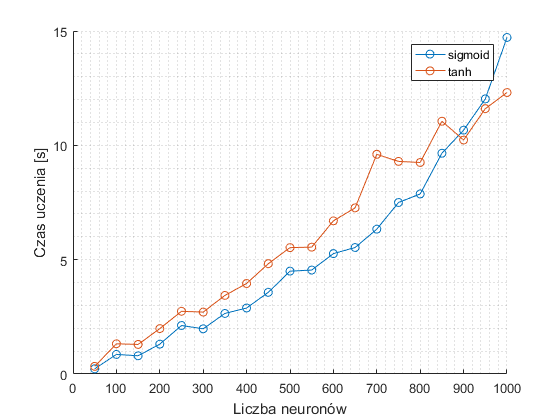
\includegraphics[width=\textwidth]{dota_wydajnosc.png}
\caption[Wykres zależności czasu uczenia od liczby neuronów]{Wykres zależności czasu uczenia od liczby neuronów (opracowanie własne)}
\label{dota_wydajnosc}
\end{figure}

\subsection{Wnioski}
\begin{itemize}
\item Sieci typu ELM są w~stanie spośród wielu kolumn danych wyłuskać oczywistą relację między niewielką liczbą cech a~wynikiem, nawet przy niewielkiej liczbie neuronów.
\item Przy prostej relacji maksymalna jakość uczenia jest osiągana przy bardzo niskiej liczbie neuronów.
\item Przy niewielkiej liczbie cech, dla liczby neuronów nieprzekraczającej znacznie 1000, długość treningu skaluje się liniowo z~liczbą neuronów. Próba dodania dużo większej liczby neuronów, na przykład 10000, znacznie spowalnia działanie i~pokazuje nieliniowość zależności.
\end{itemize}
\clearpage
\section{Klasyfikacja pokrycia lasu ze względu na dominujący gatunek drzew}
\subsection{Opis}
Benchmark polegający na klasyfikacji pokrycia lasu ze względu na dominujący gatunek drzew został dostarczony przez Jocka A. Blackarda i~Colorado State University na potrzeby konkursu zorganizowanego w~2014 roku przez Kaggle \cite{forest_cover} -- instytucję zajmującą się organizacją konkursów z dziedziny analizy danych. Obejmuje 15120 próbek, gdzie każda próbka opisuje obszar 30 na 30 metrów w~Roosevelt National Forest w~Kolorado. Próbki pochodzą jedynie z~obszarów chronionych przed działalnością człowieka w~celu wyeliminowania zewnętrznych czynników, takich jak sadzenie drzew przez ludzi. Klasyfikacja polega na przypisaniu każdemu obszarowi dominującego w~nim gatunku drzew opisanego za pomocą liczby:
\begin{enumerate}
\item świerk/jodła,
\item sosna wydmowa,
\item sosna żółta,
\item topola/wierzba,
\item osika,
\item daglezja zielona,
\item \textit{krummholz}, czyli pewna specyficzna formacja drzew różnych gatunków.
\end{enumerate}
Dane wejściowe składają się z~kolumn opisujących następujące cechy:
\begin{enumerate}
\item elewacja w~metrach,
\item kierunek nachylenia w~stopniach,
\item kąt nachylenia w~stopniach,
\item pozioma odległość od najbliższego zbiornika wodnego,
\item pionowa odległość od najbliższego zbiornika wodnego,
\item pozioma odległość od najbliższej jezdni,
\item zacienienie o~9.00 podczas przesilenia letniego,
\item zacienienie o~12.00 podczas przesilenia letniego,
\item zacienienie o~15.00 podczas przesilenia letniego,
\item pozioma odległość od najbliższego punktu podatnego na pożary,
\item 4 binarne kolumny opisujące przynależność do poszczególnych obszarów chronionych przed działalnością człowieka,
\item 40 binarnych kolumn charakteryzujących glebę.
\end{enumerate}
Dokładniejsze informacje dotyczące danych (w~tym dokładne wyjaśnienia binarnych kolumn) są dostępne na stronie będącej źródłem danych. W~tabeli \ref{forest_first_5} znajduje się 5 przykładowych próbek, z~pominięciem wspomnianych 44 kolumn binarnych.
\begin{table}[H]
\caption{Przykładowe dane dla klasyfikacji lasów}
\label{forest_first_5}
\centering
\begin{tabular}{|c|c|c|c|c|c|c|c|c|c|}
\hline
\textbf{1} & \textbf{2} & \textbf{3} & \textbf{4} & \textbf{5} & \textbf{6} & \textbf{7} & \textbf{8} & \textbf{9} & \textbf{10} \\
\hline
2596 & 51 & 3 & 258 & 0 & 510 & 221 & 232 & 148 & 6279 \\
2590 & 56 & 2 & 212 & -6 & 390 & 220 & 235 & 151 & 6225 \\
2804 & 139 & 9 & 268 & 65 & 3180 & 234 & 238 & 135 & 6121 \\
2785 & 155 & 18 & 242 & 118 & 3090 & 238 & 238 & 122 & 6211 \\
2595 & 45 & 2 & 153 & -1 & 391 & 220 & 234 & 150 & 6172 \\
\hline
\end{tabular}
\end{table}

Warto zauważyć, że dane są dosyć nietypowe, ze względu na obecność licznych kolumn binarnych, których istotność może być nawet znikoma.
\subsection{Trening sieci ELM w~Pythonie}
Aplikacja w~Pythonie osiąga dosyć niewielką skuteczność. Zarówno dla funkcji sigmoidalnej, jak i~dla tangensa hiperbolicznego, maksimum skuteczności (44\%) jest osiągane przy 1800 neuronach -- przy czym dalej procent poprawnie sklasyfikowanych próbek pozostaje na stałym poziomie, a~błąd średniokwadratowy wzrasta, co wskazuje na to, że większa liczba neuronów jedynie pogłębia różnice między klasami przypisanymi do źle przydzielonych próbek, a~oczekiwanymi rezultatami, jednocześnie nie wpływając na wynik poprawnej klasyfikacji. Co istotne, nawet dla 2400 neuronów trening potrwał jedynie 5 sekund, zgodnie z~tezą o~szybkim działaniu ELM. 
Na rysunku \ref{forest_python} zaprezentowane są wyniki dla sigmoidalnej funkcji aktywacji (grupa 1) i~tangensa hiperbolicznego (grupa 2). 

\begin{figure}[H]
\centering
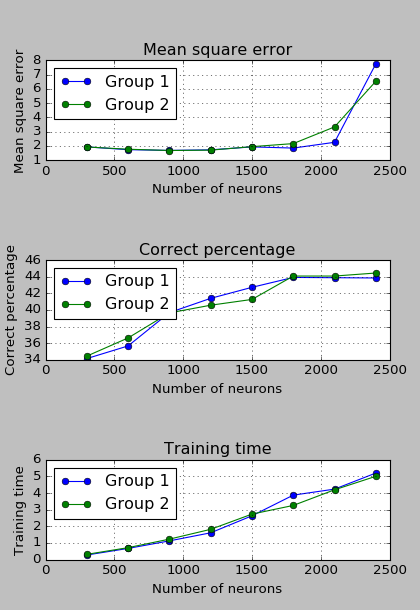
\includegraphics[width=\textwidth]{wyniki_forest_python.png}
\caption[Wyniki dla niewielkiej liczby neuronów]{Wyniki dla niewielkiej liczby neuronów (opracowanie własne)}
\label{forest_python}
\end{figure}
Patrząc na wykres czasu uczenia w~zależności od liczby neuronów, można już zauważyć, że wykres nie przedstawia linii prostej, a~krzywą, której pochodna jest rosnąca, tak więc opisany w~benchmarku z~sekcji \ref{10000_dota2} przypadek 10000 neuronów jest oczekiwaną sytuacją. Podobne rezultaty występują również dla tych danych.
\subsection{Trening sieci ELM w~Matlabie}
Przy odpowiednich parametrach aplikacja osiąga nawet do 76\% skuteczności. 
Taki wynik jest otrzymywany przy zastosowaniu 800 neuronów z~tangensem hiperbolicznym.
Przeprowadzone zostały również testy dla innych funkcji -- liniowej, sinusa, tangensa hiperbolicznego i~funkcji sigmoidalnej, a~także przy użyciu dwóch zbiorów neuronów z~różnymi funkcjami aktywacji.
Wyniki były zbliżone -- między 72\% a~76\%.

Został również zbadany wpływ liczby neuronów na jakość klasyfikacji.
Rysunek \ref{forest_liczba_neuronow} pokazuje jak zmieniała się liczba poprawnie sklasyfikowanych obiektów przy zwiększaniu liczby neuronów dla funkcji aktywacji $sigmoid$ i~$tanh$.
Jak widać w~przypadku obu funkcji jakość klasyfikacji rosła, ale coraz wolniej, aż w~końcu przestała się zmieniać.
\begin{figure}[H]
\centering
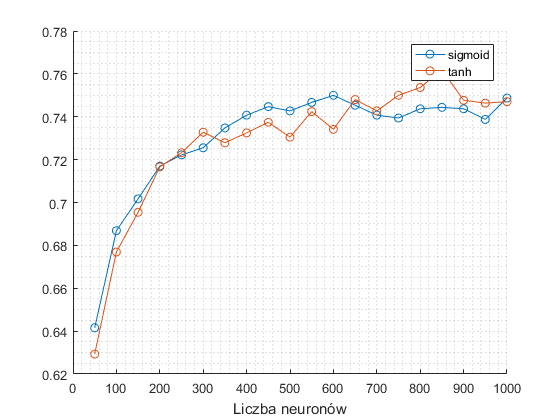
\includegraphics[width=\textwidth]{forest_liczba_neuronow.png}
\caption[Wykres zależności jakości uczenia od liczby neuronów]{Wykres zależności jakości uczenia od liczby neuronów (opracowanie własne)}
\label{forest_liczba_neuronow}
\end{figure}

Dla tych samych danych przeprowadzono testy wydajności.
Wyniki zostały przedstawione na rysunku \ref{forest_wydajnosc}.
Jak widać dla liczb neuronów, które warto rozważać (dalej nie następuje wzrost skuteczności) zależność czasu uczenia od liczby neuronów można przybliżyć do liniowej.
Uczenie nawet dla większej liczby neuronów nie trwa dłużej niż 6 sekund, co można uznać za dobry wynik.
Warto zauważyć, że użyta funkcja nie ma istotnego wpływu na czas uczenia, ponieważ głównym kosztem obliczeń jest pseudoinwersja macierzy.


\begin{figure}[H]
\centering
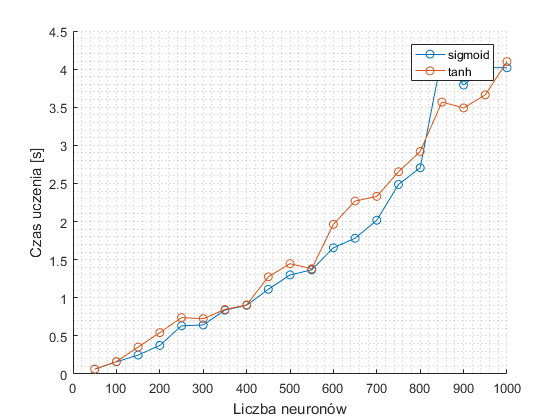
\includegraphics[width=\textwidth]{forest_wydajnosc.png}
\caption[Wykres zależności czasu uczenia od liczby neuronów]{Wykres zależności czasu uczenia od liczby neuronów (opracowanie własne)}
\label{forest_wydajnosc}
\end{figure}

Na przykładzie tego zbioru danych można zauważyć ciekawą cechę tego algorytmu -- niedeterminizm.
Występuje tu zmienny element -- losowane wagi i~wyrazy wolne.
Okazuje się, że ma to znaczący wpływ na wyniki.
Przy uruchomieniu aplikacji kilka razy dla tych samych danych wejściowych różnice w~skuteczności dochodzą nawet do 4 punktów procentowych.
Ten fakt utrudnia porównywanie funkcji aktywacji -- jedno uruchomienie nie wystarczy, żeby stwierdzić, że któraś funkcja była lepsza.

Na przykładzie powyższego zbioru danych został również przeprowadzony eksperyment, dotyczący normalizacji.
W tabeli \ref{tab_norm} zostały przedstawione wyniki klasyfikacji, przeprowadzonej dla każdej z~wybranych funkcji aktywacji dwa razy: najpierw nie korzystając, a~potem korzystając z~normalizacji.
Można zauważyć, że jedynie dla funkcji liniowej wyniki są porównywalne.
W przypadku pozostałych funkcji zrezygnowanie z~normalizacji pogarsza skuteczność od 3 aż do 5 razy.
W przypadku funkcji Gaussa, osiągającej dobry wynik przy zastosowaniu normalizacji, skuteczność uczenia bez jej zastosowania jest porównywalna z~losową klasyfikacją.
\begin{table}[H]
\caption{Skuteczność (w~procentach) klasyfikacji z~normalizacją i~bez dla przykładowych funkcji aktywacji}
\label{tab_norm}
\begin{tabular}{|l|c|c|c|c|c|}
\hline
& $x$ & $sin(x)$ & $\frac{1}{1+e^{-x}}$ & $tanh(x)$ & $e^{-x^2}$ \\
\hline
\textbf{Bez normalizacji} & 65 & 16 & 23 & 21 & 13 \\
\hline
\textbf{Z normalizacją} & 63 & 68 & 69 & 66 & 67 \\
\hline

\hline
\end{tabular}
\end{table}
Można wywnioskować, że w~tej implementacji zastosowanie normalizacji jest koniecznością.
Jako że polega ona na zastosowaniu jedynie kilku prostych operacji arytmetycznych na macierzy, jej koszt jest bardzo niewielki -- pomijalny w~stosunku do czasu trwania całego algorytmu.

Wyniki można uznać za zadowalające -- skuteczność jest całkiem wysoka, a~czas uczenia niski.
Dzięki temu, że dane pochodzą z~konkursu Kaggle, można porównać otrzymany wynik z~nadesłanymi rozwiązaniami.
Uzyskany rezultat plasuje się około pięćsetnego miejsca na 1694 nadesłane odpowiedzi.
Można to uznać za sukces tej metody, jeśli wziąć pod uwagę dwa fakty.
Po pierwsze algorytm nie był w~żaden sposób optymalizowany pod kątem tych danych, co prawdopodobnie miało miejsce w~przypadku większości przesłanych odpowiedzi.
Po drugie w~konkursie nie było wymagań związanych z~czasem uczenia, więc można było zastosować wolniejsze, ale skuteczniejsze metody.
\subsection{Wnioski}
\begin{itemize}
\item Dla dużej liczby cech, przy liczbach neuronów nieprzekraczających znacząco 1000, podobnie jak dla omawianego wcześniej przypadku mniejszej liczby cech, czas treningu jest liniowy. Przy większej liczbie neuronów widać już, że liniowość relacji była jedynie pozorna, a~w rzeczywistości wykres przedstawia krzywą rosnącej pochodnej.
\item Wyniki implementacji ELM z~biblioteki \textit{HP-ELM} znacząco się różnią od wyników własnej implementacji w~Matlabie, która została stworzona jako bezpośrednie wdrożenie opisanej wcześniej części teoretycznej -- co sugeruje, że istnieją między nimi znaczące różnice. Znanymi różnicami między aplikacją w~Pythonie i~Matlabie jest normalizacja (w~Matlabie własna, a~w Pythonie została użyta w~tym celu biblioteka \textit{sklearn}) oraz sposób losowania wag (w~Matlabie wykorzystany rozkład normalny, w~\textit{HP-ELM} nie została podana metoda losowania). Jeśli różnice w~otrzymanych rezultatach nie są wynikiem którejś z~powyższych rozbieżności, sugerowałoby to, że implementacja \textit{HP-ELM} zawiera odstępstwa od teorii -- jednak najprawdopodobniej najistotniejszym czynnikiem powodującym różnice są wskazane kwestie, nieuwzględnione w~części teoretycznej.
\end{itemize}
\clearpage
\chapter*{Podsumowanie}
%\addcontentsline{toc}{chapter}{Podsumowanie}
Na podstawie eksperymentów przeprowadzonych przy użyciu obu aplikacji można wyciągnąć wnioski dotyczące sieci ELM, a~także detali implementacji.

Uzyskane rezultaty są zgodne z~wnioskami przedstawionymi w~cytowanych pracach.
Uczenie jest szybkie i~skuteczne.
Warto jednak zauważyć, że zwiększanie liczby neuronów dość szybko przestaje poprawiać rezultaty, a~coraz bardziej zwiększa czas uczenia.

Istnieją znaczne różnice między wynikami aplikacji w~Matlabie i~Pythonie. Ta pierwsza jest skuteczniejsza, ale druga jest szybsza. Pokazuje to, że niewielkie różnice w~implementacji (rozdział \ref{porownanie_aplikacji}) znacznie zmieniają działanie aplikacji.

Prowadzi to do kolejnego wniosku -- istnieją niesprecyzowane w~pracach detale algorytmu, które mogą zauważalnie wpłynąć na wyniki.
Należą do nich:
\begin{itemize}
\item sposób normalizacji danych, 
\item metoda losowania wag wejściowych,
\item funkcje aktywacji.
\end{itemize}
Możliwe są dalsze eksperymenty, sprawdzające różne warianty implementacji ELM, być może prowadzące do jeszcze lepszych wyników.
\clearpage




% 6. Bibliografia
% Bibliografia leksykograficznie wg nazwisk autorów

\begin{thebibliography}{20}%jak ktoś ma więcej książek, to niech wpisze większą liczbę
% \bibitem[numerek]{referencja} Autor, \emph{Tytuł}, Wydawnictwo, rok, strony
% cytowanie: \cite{referencja1, referencja 2,...}

\bibitem{akusok-hpelm}
  A. Akusok, K.-M. Björk, Y. Miche, A. Lendasse,
  \emph{High-Performance Extreme Learning Machines: A~Complete Toolbox for Big Data Applications.}
  IEEE Access 3 (2015): 1011-1025.

\bibitem{huang-elm-base}
  A. G.-B. Huang, L. Chen, C.-K. Siew, 
  \emph{Extreme Learning Machine: A~new Learning Scheme of Feedforward Neural Networks.}
   Neural Networks, 2004. Proceedings. 2004 IEEE International Joint Conference on. Vol. 2. IEEE, 2004.

\bibitem{huang-elm-rbf}
  A. G.-B. Huang, C.-K. Siew, 
  \emph{Extreme Learning Machine: RBF Network Case.} 
  Control, Automation, Robotics and Vision Conference, 2004. ICARCV 2004 8th. Vol. 2. IEEE, 2004.

\bibitem{huang-elm-tap}
  A. G.-B. Huang, L. Chen, C.-K. Siew, 
  \emph{Extreme Learning Machine: Theory and Applications.} 
  Neurocomputing 70.1 (2006): 489-501.
  
\bibitem{originofelm} 
  ELM Origin,
  \emph{http://elmorigin.wixsite.com/originofelm.}
  Accesed: 23 October 2016.
  
\bibitem{hpelm}
  HP-ELM library on github,
  \emph{https://github.com/akusok/hpelm}
   Accesed: 30 October 2016.

  
\bibitem{hdf5}
  The HDF Group,
  \emph{https://support.hdfgroup.org/HDF5/} 
  Accesed: 15 November 2016.
 
  
\bibitem{h5py}
  HDF5 for Python documentation,
  \emph{http://www.h5py.org/}
  Accesed: 19 November 2016.

\bibitem{numpy}
  Numpy documentation,
  \emph{http://www.numpy.org/}
  Accesed: 8 October 2016.  
  
\bibitem{sklearn}
  Scikit-learn documentation,
  \emph{http://scikit-learn.org/}  
  Accesed: 10 October 2016.
  
\bibitem{dota2}
  Kaggle,
  \emph{https://www.kaggle.com/devinanzelmo/dota-2-matches}
  Accesed: 3 January 2017.
  
\bibitem{dota2_webapi}
  Dota 2 WebAPI,
  \emph{https://wiki.teamfortress.com/wiki/WebAPI/GetMatchDetails}
  Accesed: 3 January 2017.
  
\bibitem{dota2_map_src}
  Dota 2 Wiki,
  \emph{http://dota2.gamepedia.com/File:Labelled\textunderscore Map.png}
  Accesed: 10 January 2017.

\bibitem{forest_cover}
  Kaggle,
  \emph{https://www.kaggle.com/c/forest-cover-type-prediction/data}
  Accesed: 12 December 2016.

\end{thebibliography}



% 7. Wykaz symboli i skrótów - jeśli nie ma, zakomentować
\chapter*{Wykaz symboli i skrótów}

\begin{tabularx}{\textwidth}{cX}
\textbf{Benchmark} & test wydajności i~jakości treningu \\
\textbf{Bias} & wyraz wolny, czyli dodatkowy neuron w~warstwie wejściowej niewynikający z~danych wejściowych, generujący zawsze +1, ale posiadający wagę \\
\textbf{Big Data} & dane z~liczbą próbek tak dużą, że nie występuje efekt przeuczenia w~klasycznych sieciach neuronowych; dane, nie mieszczące się w~całości w~pamięci RAM \\ 
\textbf{BP} & \textbf{B}ack-\textbf{p}ropagation -- propagacja wsteczna \\ 
\textbf{ELM} & \textbf{E}xtreme \textbf{L}earning \textbf{M}achine -- ekstremalne uczenie maszynowe \\ 
\textbf{GPU} & \textbf{G}raphics \textbf{P}rocessing \textbf{U}nit -- procesor graficzny \\ 
\textbf{MLP} & \textbf{M}ulti\textbf{l}ayer \textbf{P}erceptron -- perceptron wielowarstwowy \\ 
\textbf{RBF} & \textbf{R}adial \textbf{B}asis \textbf{F}unction -- radialna funkcja bazowa, czyli funkcja rzeczywista, której wartość zależy tylko od odległości od pewnego punktu \\ 
\textbf{SLFN} & \textbf{S}ingle-\textbf{L}ayer \textbf{F}eed-forward \textbf{N}etwork -- jednowarstwowa jednokierunkowa sieć neuronowa \\ 
\textbf{Small Data} & dane, dla których jest za mało próbek, aby klasyczna sieć poznała dokładnie model bez przeuczenia; mieszczące się w~pamięci RAM \\ 
\textbf{SVM} & \textbf{S}upport \textbf{V}ector \textbf{M}achine -- maszyna wektorów nośnych \\ 
\textbf{Toolbox} & zbiór funkcji stworzonych we wspólnym celu; biblioteka \\ 
\end{tabularx}


% 8. Spis rysunków - jeśli nie ma, zakomentować (ale być może po prostu się nie zrobi)
\listoffigures


% 9. Spis tabel - jak wyżej
\listoftables


% 10. Spis załączników - jak nie ma załączników, to zakomentować lub usunąć
\chapter*{Spis załączników}
\begin{enumerate}
\item[1.] Załącznik 1
\item[2.] Załącznik 2
\end{enumerate}

% 11. Załączniki
\chapter*{Dodatek. Instrukcja obsługi aplikacji}
%\addcontentsline{toc}{chapter}{Dodatek. Instrukcja obsługi aplikacji}
\section*{Aplikacja sieci ELM w~Pythonie}
\subsection*{Przygotowanie}
Aplikacja sieci ELM w~Pythonie wymaga zainstalowania najnowszej wersji Pythona 2 wraz ze standardowymi bibliotekami -- najprostszym sposobem jest zainstalowanie pakietu Anaconda. Oprócz tego, należy zainstalować bibliotekę \textit{HP-ELM} -- należy uruchomić konsolę z~uprawnieniami administratora i~wywołać polecenie \textit{pip install hpelm}. 
\subsection*{Uruchomienie aplikacji}
Aby uruchomić aplikację, należy za pomocą folderu przejsć do katalogu zawierającego pliki aplikacji i~wywołać polecenie \textit{python test.py}. W~przypadku niektórych systemów operacyjnych (na przykład Arch Linux) może być konieczne użycie zamiast tego polecenia \textit{python2 test.py}.
\clearpage
\subsection*{Użytkowanie aplikacji}
Bezpośrednio po uruchomieniu powinien pojawić się ekran jak na rysunku \ref{python_ekran}.
\begin{figure}[H]
\centering
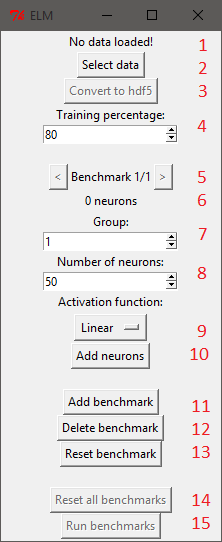
\includegraphics[width=0.4\textwidth]{instrukcja_python_start.png}
\caption[Ekran aplikacji]{Ekran aplikacji (opracowanie własne)}
\label{python_ekran}
\end{figure}
Zawiera elementy oznaczone tu liczbami od 1 do 15:
\begin{enumerate}
\item nazwa załadowanego pliku z~danymi,
\item wybór danych -- uruchamia dwa okienka umożliwiające wybór pliku z~danymi w~formacie \textit{csv} (dla small data) i~\textit{hdf5} (dla big data) -- pierwsze okienko to wybór danych wejściowych, a~drugie okienko to wybór oczekiwanych wyników,
\item konwersja wczytanych danych do \textit{hdf5} -- pozwala na utworzenie plików \textit{hdf5} zgodnych z~aplikacją, na przykład w~celu zasymulowania obliczeń big data,
\item procent danych treningowych,
\item obecnie wybrany benchmark oraz kontrolki pozwalające przełączać się między benchmarkami,
\item liczba neuronów w~obecnym benchmarku,
\item grupa, do której należy obecny benchmark,
\item liczba neuronów do dodania do obecnego benchmarku,
\item funkcja aktywacji dla neuronów do dodania do obecnego benchmarku,
\item dodanie określonych powyżej neuronów,
\item dodanie nowego benchmarku (przypisanego do tej samej grupy, co obecny benchmark),
\item usunięcie obecnego benchmarku,
\item usunięcie wszystkich neuronów z~obecnego benchmarku,
\item usunięcie wszystkich benchmarków,
\item uruchomienie benchmarków.
\end{enumerate}
Aby skorzystać poprawnie z~aplikacji, należy najpierw wybrać dane, ustalić procent danych treningowych, dodać tyle benchmarków, ile się chce (w~każdym musi być co najmniej jeden neuron), przypisać im odpowiednie grupy, aby podzielić otrzymane wyniki na różne serie danych, a~następnie wcisnąć przycisk \textit{Run benchmarks}. Efektem jest pojawienie się nowego okienka z~wykresami opisującymi wyniki eksperymentu, jak na rysunku \ref{instrukcja_python_end}.
\begin{figure}[H]
\centering
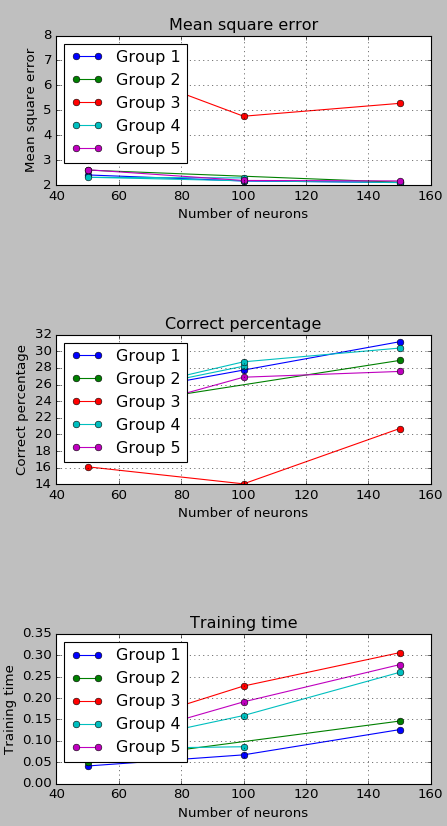
\includegraphics[width=0.8\textwidth]{instrukcja_python_end.png}
\caption[Przykładowe wyniki działania aplikacji]{Przykładowe wyniki działania aplikacji (opracowanie własne)}
\label{instrukcja_python_end}
\end{figure}
\clearpage
\section*{Aplikacja sieci ELM w~Matlabie}
\subsection*{Przygotowanie}
Aby uruchomić aplikację, należy skorzystać z~programu Matlab.
Aplikacja składa się z~dwóch plików: klasy sieci, zawierającej implementację algorytmu (\textit{ELM.m}) i~przykładowego skryptu wywołującego kolejne funkcje tej klasy (\textit{ELM\textunderscore run.m}).
Konieczne jest ustawienie folderu roboczego na folder, w~którym znajdują się te pliki.
\subsection*{Użytkowanie aplikacji}
Uruchomienie aplikacji polega na wywołaniu skryptu \textit{ELM\textunderscore run.m}, jednak najpierw należy ustawić wszystkie konieczne parametry. Rysunek \ref{elm_run} przedstawia kod skryptu \textit{ELM\textunderscore run.m} z~pominięciem części odpowiedzialnej za komunikację z~użytkownikiem.
\begin{figure}[H]
\centering
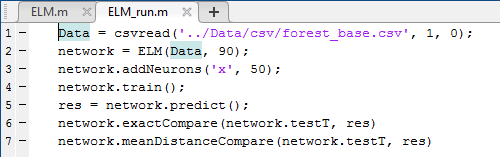
\includegraphics[width=1\textwidth]{elm_run.png}
\label{elm_run}
\caption[Skrypt \textit{ELM\textunderscore run.m}]{Skrypt \textit{ELM\textunderscore run.m} (opracowanie własne)}
\end{figure}
Znaczenie i~możliwe modyfikacje kolejnych linii:
\begin{enumerate}
\item Przygotowanie danych wejściowych.
W tym wypadku dane są wczytywane z~pliku csv, co nie jest konieczne.
Wymagane jest jedynie, żeby dane wejściowe następnej funkcji były macierzą, w~której $n$ kolumn oznacza cechy, a~jedna (ostatnia) klasy, do których należą próbki. Wartości wszystkich cech i~klas muszą być liczbami.
\item Konstruktor klasy sieci. 
Pierwszy argument to wspomniana wcześniej tablica. 
Drugi oznacza procent danych przeznaczonych do treningu sieci.
Pozostałe dane (w~tym wypadku 10\%) to dane testowe.
\item Dodawanie neuronów.
Pierwszy argument to funkcja aktywacji.
Może to być dowolny kod wykonywalny w~Matlabie, gdzie zmienną jest x.
Drugi argument to liczba neuronów tego typu.
Ta funkcja może zostać wywołana dowolnie wiele razy, aby stworzyć neurony o~różnych funkcjach aktywacji.
\item Rozpoczęcie treningu sieci. 
Funkcja wykorzystuje dane wybrane w~drugim kroku jako treningowe.
Należy ją wywołać po dodaniu wszystkich neuronów.
\item Klasyfikacja danych testowych.
Wynikiem jest wektor klas -- po jednej dla każdego obiektu, należącego do danych testowych.
\item Funkcja porównująca wynik uzyskany w~poprzednim kroku z~oczekiwaniami.
Przyjmuje jako argumenty wektor z~danymi oczekiwanymi (zapisany wcześniej przez aplikację jako pole klasy) i~wektor wynikowy klasyfikacji.
Funkcja zwraca liczbę z~zakresu $[0, 1]$, oznaczającą jaka część próbek została sklasyfikowana poprawnie.
\item Inna funkcja poprawności klasyfikacji, przyjmująca takie same argumenty.
Zwraca średnią odległość klas przewidzianych od faktycznych.
Ta miara może być użyteczna, jeśli klasy o~bliskich numerach są bardziej zbliżone niż o~dalekich.
\end{enumerate}
Po odpowiednim zmodyfikowaniu skryptu i~uruchomieniu go otrzymujemy wynik (rys. \ref{elm_run_result}) -- informacje o~czasie trwania i~skuteczności treningu.
\begin{figure}[H]
\centering
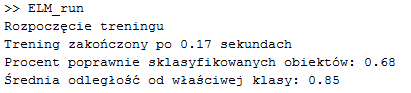
\includegraphics[width=0.9\textwidth]{elm_results.PNG}
\caption[Wynik wywołania skryptu]{Wynik wywołania skryptu (opracowanie własne)}
\label{elm_run_result}
\end{figure}
\end{document}



















